\section{Description of Tool}
\label{sec:tool}

\begin{figure}[ht]
  \centering
  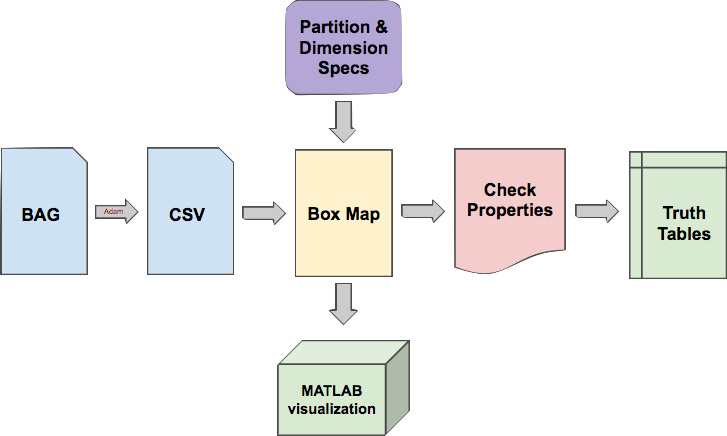
\includegraphics[width=0.95\textwidth]{./figures/workflow}
  \caption{Overview of tool workflow.}
  \label{fig:workflow}
\end{figure}

 \begin{itemize}
  \item \emph{Input}: 
   \begin{itemize}
    \item One or more .bag files of ROS message data containing positional data and time stamps
    \item A flag to indicate a single entity or multiple entities
    \item Partition specifications given as a 3-tuple of positive integer values
    \item Dimension specifications (in meters) given as a 3-tuple of positive floating-point values
   \end{itemize}

  \item \emph{Output}:
   \begin{itemize}
    \item Visualization in MATLAB of entity's/entities' movement through space
    \item Truth table(s) with the following properties:
      \begin{itemize}
       \item moves? : occupies more than one box
       \item returns home? : occupies the initial box in separate time intervals
       \item box independence? : multiple entities (traces, given a single entity) never occupy the same box simultaneously
       \item crumb independence? : multiple entities (traces, given a single entity) never cross each other's box-path
       \item fuzzy box independence? : multiple entities (traces, given a single entity) never occupy the same "fuzzy" box simultaneously
       \item fuzzy crumb independence? : multiple entities (traces, given a single entity) never cross each other's "fuzzy" box-path
       \item returns to some box? : occupies the same box in separate time intervals
       \item loiters? : remains in the same box for more than 30 seconds
      \end{itemize}

   \end{itemize} 
 \end{itemize}
 
 For many of the above properties, it will be important to know specific details of violated properties (which box, which time frame, etc.); these details are being stored but we are currently only outputting binary truth values. 
 
 This description elaborates on the high-level workflow diagram.
 We first convert the .bag files to .csv files with four columns which contain a timestamp and the associated x, y, and z position values (in meters).  
 Our tool currently makes the assumption that we receive one \emph{complete} trace of some run, so we are not stitching together partitions of lengthy runs; this may need to be done in the future.
 Each time frame is mapped to some box, so to temporally sync the runs, we are considering the start of the run to be the global time frame of the greatest initial time frame of all given traces.
 
 Given the dimensions and desired partition specifications, we map the position of each time frame of a single trace to the box corresponding to its position.
 This produces a total ordering of abstracted trace positions given as a succession of boxes, which we will call a box-trace.
 
 Based on a set of box-traces, we will check if certain properties hold.
 For example, if a trace starts out in "box 3," moves to other boxes, and occupies "box 3" at a later time, then the return home property would be set to true.
 
 Let there be $m$ properties.
 If we are considering a single entity, the truth table will just be one row with $m$ columns containing the truth value of the corresponding property.
 If we are considering $n$ multiple entities, the output will be $m$ truth tables which are either $1 \times n$ or $n \times n$ matrices, depending on the property considered.
 For example, the returns home property only depends on a single entity, not their interactions, so the table will be a $1 \times n$ matrix with the truth value of each entity.
 But a property like box-independence considers interactions between all the entities, and so its truth table will be a $n \times n$ matrix with the truth value for box-independence between $(box_i,box_j)$ for all $1 \leq i,j \leq n$.
